\chapter{Algorithmic Approaches}
\label{cha:algorithmic} % (labels for cross referencing)

\section{The Bernoulli Bandit Vs The Gaussian Bandit}
\label{sec:BernoulliBandit}

The Bernoulli bandit problem and the Gaussian bandit problem are both sequential decision-making problems:

In the Bernoulli bandit, the rewards are drawn from a Bernoulli distribution of unknown mean, which manifests as a binary result between two possible outcomes (normally success or failure). The goal is to select arms in a strategic manner to maximize the cumulative reward. This should balance exploration to learn more about other arm's expected means and exploitation of the best-performing arms.

In contrast, the Gaussian bandit involves rewards drawn from a Gaussian distribution with unknown variance and mean, that manifests as a continuous outcome between [0, 1]. The objective is identical to the Bernoulli bandit, but the focus is on estimating unknown means and using information to make optimal decisions.

\subsection{Algorithmic Approaches}
\label{sec:Algorithms}

\subsubsection{Randomized}
\label{sec:randomized}
The randomized algorithm for multi-armed bandits involves selecting arms at random with equal probability, without considering any feedback or past performance. This algorithm is commonly referred to as the "purely random" or "uniform random" algorithm.

The random algorithm can be summarized as follows:

\pseudobox{%
  \KwIn{List of arms $\armsList$ with unknown distributions $\armDistributionVect$, number of timesteps $\timeHorizon$}
  \KwOut{Selection strategy}

  \BlankLine
  \For{$t = 1,\ldots, \timeHorizon$}{
    Choose a random arm $A_t$ uniformly from the set of arms $1,2,\ldots,K$;\newline
    Receive the reward $\reward{t}{}$ by pulling arm $A_t$;
  }
}{Randomized Algorithm}

At each time step $t$, the Randomized algorithm randomly selects an arm $A_t$ from K arms, following a uniform distribution:

$$\text{For } i \in \{1, 2, \ldots, K\}: \Prob(A_t = i) = \frac{1}{K}$$

This algorithm is quite often used as a baseline for more sophisticated algorithm evaluation. In the long run, the average reward converges towards the discrepancy between the maximum and the average reward. More precisely, by the strong law of large numbers the following holds almost surely,

$$\lim_{{t \to \infty}} \frac{1}{t}\cdot \cumulativeRegret{t}{\policy} = \maxPopulationMean-\frac{1}{\numArms} \sum_{{k=1}}^{\numArms} \armPopulationMean{k}.$$

Although this algorithm is very simple to implement, it doesn't attempt to optimize arm selection based on past events. It can be described as a purely exploratory algorithm that doesn't exhibit any exploitative behavior, hence its performance is generally vastly inferior to that of any other algorithms.

\subsubsection{Greedy}
\label{sec:Greedy}
The Greedy algorithm is a step-up from randomly picking arms, since it actually takes into account past performance. Put simply, it chooses the arm that has the highest estimated expected reward, denoted by the arm with the highest current rate of success.

To begin, it assigns each arm with a "action-value estimate" \actionValueEstimate, essentially the predicted success rate of each arm. This is often set arbitrarily at some value, usually 0.5 or 1.

Then, at each time step $t$, the Greedy algorithm selects the arm $A_t$ with the highest expected success rate.

The Greedy algorithm can be summarized as follows:

\pseudobox{%
    \KwIn{List of arms $\armsList$ with unknown distributions $\armDistributionVect$, action-value estimate \actionValueEstimate, number of timesteps $\timeHorizon$}
    \KwOut{Selection strategy}
    \BlankLine
    \ForEach{arm $i = 1$ \KwTo $K$}{
        Initialise success rate $Q_i \leftarrow $\actionValueEstimate\newline
        Initialise number of successes $S_i \leftarrow \mathcal{0}$\newline
        Initialise count $C_i \leftarrow 0$
    }
    \BlankLine
    \For{$t = 1,\ldots, \timeHorizon$}{
        Choose arm $A_t = a$ with the highest success rate: $a \leftarrow \arg\max_i Q_i$\newline
        Receive the reward $R_t$ by pulling arm $a$;\newline
        Increment count: $N_a \leftarrow N_a + 1$\newline
        Increment successes: $S_a \leftarrow S_a + R_t$\newline
        Update success rate: $Q_a \leftarrow \frac{S_a}{N_a}$

  }
}{Greedy Algorithm}

Although this algorithm is simple and fast, it tends to exploit the immediate best option, and very rarely explores other options to try and optimise it's rewards.

Moreover, the value of \actionValueEstimate \space can significantly impact the algorithm's performance - in the extreme case where \actionValueEstimate=0, the algorithm will keep pulling the first arm that succeeds, preventing any further exploration.
In a practical sense, when implementing this in code, it could explore other arms when the programming language registers the success rate as so low it rounds down to 0.
For example, Python will do this only when the success rate goes below $10^{-324}\%$ \cite{python_min_float}.

However, the Greedy algorithm can exhibit linear regret under general conditions: consider a 2-arm bandit with arms 0.9 and 0.8. Employing the Greedy algorithm may lead to linear regret, if it gets unlucky and gets a miss on arm 1, and a hit on arm 2, with probability 8\%. This essentially locks the algorithm into choosing this sub-optimal arm, and as a result, it could miss out on the higher reward arm, leading to persistent linear regret.

\subsubsection{Epsilon Greedy}
\label{sec:EpsilonGreedy}
The Epsilon Greedy algorithm is a combination of the Greedy and Randomized algorithm, addressing their tendencies to over-exploit and over-explore. It introduces a trade-off by incorporating an additional parameter $\epsilon$.

The core of the Epsilon Greedy algorithm is the same action-value estimate for each arm, as described in the Greedy algorithm. However, instead of always selecting the arm with the highest estimated success rate, the Epsilon Greedy algorithm randomly explores other arms with the hope of finding potentially better options. This choice is determined by sampling a Bernoulli distribution based on a probability of doing something random \epsilonFunction, which varies as a function of time $t$. Usually, this is either constant, linearly decreasing, or constant with a drop to 0.


The algorithm can be summarized as follows:

\pseudobox{%
    \KwIn{List of arms $\armsList$ with unknown distributions $\armDistributionVect$, action-value estimate \actionValueEstimate, number of timesteps $\timeHorizon$, sequence of exploration rates $(\epsilon_t)_{t \in [\timeHorizon]}$}
    \KwOut{Selection strategy}
    \BlankLine
    \ForEach{arm $i = 1$ \KwTo $K$}{
        Initialise success rate $Q_i \leftarrow $\actionValueEstimate\newline
        Initialise number of successes $S_i \leftarrow \mathcal{0}$\newline
        Initialise count $C_i \leftarrow 0$
    }
    \BlankLine
    \For{$t = 1,\ldots, \timeHorizon$}{
        \If{\epsilonFunction}{
            Choose a random arm $A_t \leftarrow$ Randomized(K)
        }
        \Else{
            Choose arm $A_t = a$ with the highest success rate: $a \leftarrow \arg\max_i Q_i$
        }
        Receive the reward $R_t$ by pulling arm $A_t$\newline
        Increment count: $N_{A_t} \leftarrow N_{A_t} + 1$\newline
        Increment successes: $S_{A_t} \leftarrow S_{A_t} + R_t$\newline
        Update success rate: $Q_{A_t} \leftarrow \frac{S_{A_t}}{N_{A_t}}$

}
}{Epsilon Greedy Algorithm}

Small \epsilonFunction \space values results in a more greedy strategy where the algorithm primarily exploits the current best arm. Conversely, a larger  \epsilonFunction \space values increases exploration and encourages the algorithm to try different arms more frequently.

While the Epsilon Greedy algorithm can mitigate the issues of the Greedy and Randomized algorithm, it is not without its shortcomings - set the exploration rates in \epsilonFunction \space too low, and the algorithm may get stuck in local sub-optimal arms and miss out on potentially better arms. On the other hand, too high values of \epsilonFunction \space means it might spend too much time exploring and not enough time exploiting the best arms, leading again to sub-optimal performance.

The Epsilon-Greedy algorithm can also exhibit linear regret under general conditions: consider a 2-arm bandit with arms 0.9 and 0.4, with a fixed exploration rate \epsilonFunction \space = 0.5 $\forall t$. This initial randomness causes persistent reliable frequent sub-optimal selections, even as the algorithm learns and favors the better arm. The initial exploration-induced regret persists, resulting in an overall linear regret growth no less than (0.9 - (0.9+0.4)/2) = 0.25 per time-step. A good rule of thumb to follow is to never, in the long run, have \epsilonFunction $> \frac{1}{\numArms} - \frac{1}{\numArms^2}$, since this will cause the algorithm to, at worst, behave purely greedily


\subsubsection{Upper Confidence Bound (UCB)}
\label{sec:UCB}

% https://www.jmlr.org/papers/volume3/auer02a/auer02a.pdf

The Upper Confidence Bound algorithm (UCB) is a popular MAB algorithm that cleverly modifies the exploration rate using the confidence bounds around each arm. This helps UCB estimate how likely an arm is to succeed, while factoring in how uncertain we are about this estimate.

The key idea is to choose arms that might give high rewards, while considering the uncertainty around their success rates. At each step, UCB selects the arm that strikes the best balance between exploiting its success rate and exploring its confidence bound.

\begin{figure}[ht]
    \centering
    \makebox[\textwidth]{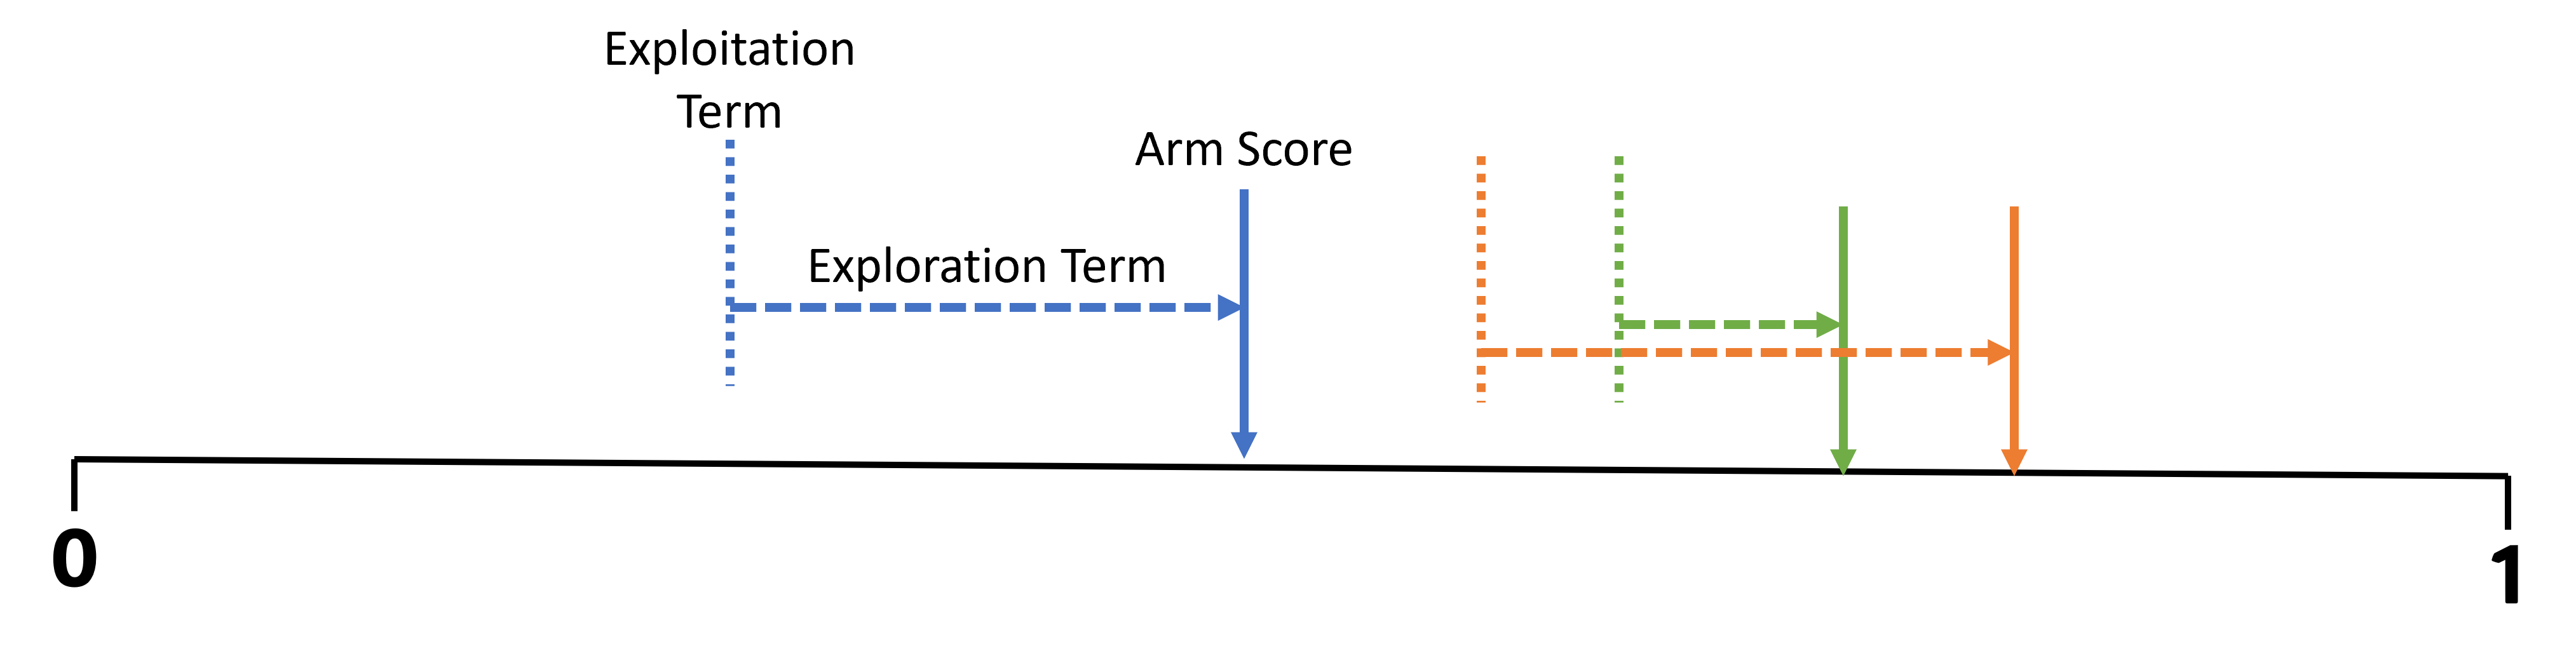
\includegraphics[width=1\textwidth]{report/images/UCB Image.png}}
    \caption{A Visual Aid to the UCB Algorithm}
    \label{fig:ucb_image}
\end{figure}



In general terms, any UCB algorithm can be described by:

$$
A_t = \arg\max_i \left[ \text{exploitation term} + \text{exploration term} \right]
$$

where the exploration term usually tends to zero as $t \rightarrow \infty$. For example, in the above figure \ref{fig:ucb_image}, the exploitation term is an indication of how "good" the arm is, whereas the exploration term is usually a measure of how unsure we are of the arm. Even though the \contour{green}{green} arm has a higher exploitation score, the \contour{orange}{orange} arm has more uncertainty around it, hence it's exploration score is higher 

More specifically in this project, we will use the UCB1 algorithm \cite{Slivkins_2019}, which uses this formula:

$$
A_t = \arg\max_i \left( Q_i +  \sqrt{\frac{c\log(t)}{N_i}} \right)
$$

For some confidence value $c$. We use $c = 2$ for optimal regret. This allows us to derive the sensible confidence bounds, since it gives a probabilistic guarantee of how likely our sample mean is to deviate from the true mean of an arm distribution.

For UCB, finite sample concentration inequality-based (FSCI) confidence intervals are preferred over Central Limit Theorem (CLT) confidence intervals due to their better performance when handling small sample sizes. CLT-based intervals rely on the assumption of having a large sample size (which ensures the sample mean converges to a normal distribution). However, in MAB problems, we sometimes have very limited data for some/all arms.

In contrast, FSCI-based confidence intervals such as Hoeffding's inequality, give bounds on the deviation of the sample mean from the true mean with high probability, even with very small sample sizes. This helps account for the inherent randomness of MAB, and the exploration-exploitation trade-off, as arms that have a poor sample mean calculated from very few attempts still have a good-enough guess for their true mean.

The algorithm can be summarized as follows:

\pseudobox{%
    \KwIn{List of arms $\armsList$ with unknown distributions $\armDistributionVect$, confidence value $c$, number of timesteps $\timeHorizon$}
    \KwOut{Selection strategy}
    \BlankLine
    \ForEach{arm $i = 1$ \KwTo $K$}{
        Initialise success rate $Q_i \leftarrow $\actionValueEstimate\newline
        Initialise count $N_i \leftarrow 0$
    }
    \BlankLine
    \For{$t = 1,\ldots, \timeHorizon$}{
        Choose arm $A_t \leftarrow \arg\max_i \left( Q_i + \sqrt{\frac{c\log(t)}{N_i}} \right)$\;
        Receive the reward $R_t$ by pulling arm $A_t$\;
        Increment count: $N_{A_t} \leftarrow N_{A_t} + 1$\;
        Update success rate: $Q_{A_t} \leftarrow \frac{S_{A_t}}{N_{A_t}}$
    }
}{Upper Confidence Bound (UCB) Algorithm}

In the UCB algorithm, it aims to balance the exploitation of arms with high estimated success rates and the exploration of arms with high uncertainty or limited exploration history:

\begin{itemize}
    \item $Q_i$ chooses greedily which arm to pick given their past success rates
    \item $\sqrt{\frac{c\log(t)}{N_i}}$ attempts to sway the greedy exploration, by adding some uncertainty to the result.
    \begin{itemize}
        \item If an arm hasn't been pulled very often, the uncertainty is very large, and vice versa. Therefore, over time, the algorithm becomes more and more `confident' about it's estimates.
        \item Due to the logarithmic nature of this particular uncertainty term, it'll slowly increase when arms aren't selected, but quickly shrink when they are. Therefore, the algorithm will tend to not `give up' on arms that appear to be sub-optimal, and will pull them infrequently until a significant score is obtained by another arm.
    \end{itemize}
\end{itemize}

One of the key advantages of UCB is that it naturally adapts its exploration strategy over time. As the algorithm collects more data and gains confidence in the success rates of different arms, the exploration bonus diminishes, leading to a more exploitation-focused strategy. In comparison to the previous algorithms, UCB offers a more systematic approach to exploration by considering uncertainty explicitly. Depending on the problem at hand, UCB can provide a more efficient trade-off between exploration and exploitation, potentially leading to better overall performance in various applications.

The regret bound for the UCB $\policy$ is sub-linear. Indeed, the rate is $O(\sqrt{n})$.

Finally, given a failure probability $\delta \in (0,1)$, we let $\ucb{a}{t}{\delta}$ denote the upper confidence bound on $\armPopulationMean{a}$ based on the first $t$ rounds,


\begin{theorem}[UCB regret bound]\label{thm:ucbRegretBound}
Suppose we have a stochastic bandit problem with time horizon $\timeHorizon \in \N$ and $\numArms \in \N$ with corresponding gaps $(\gap{i})_{i \in [\numArms]}$. Then letting $\ucbPolicy$ be the UCB policy with parameters $\delta$, $\totalFunction{a}{t}$ and $\empiricalMeanReward{a}{t}$, we have the following regret bound,
\begin{align*}
\cumulativeRegret{T}{\ucbPolicy} \leq 8 \sqrt{\timeHorizon \numArms \log(\timeHorizon)} + 3 \sum_{i=1}^{\numArms} \gap{i}.
\end{align*}
\end{theorem}

We shall now give a high-level description of the proof from this paper \cite{Lattimore_Szepesv´ar}. Recall that $\totalFunction{i}{\timeHorizon}$ denotes the number of times arm $i \in [\numArms]$ has been played over the time horizon $\timeHorizon$. We break down the regret for the UCB policy,

\begin{align}\cumulativeRegret{T}{\ucbPolicy} \leq \sum_{i=1}^{\numArms} \gap{i} \cdot \Ex(\totalFunction{i}{\timeHorizon}). \label{eq:ucb-breakdown}
\end{align}

Using the Law of Total Expectation, we can split up the $\Ex(\totalFunction{i}{t})$ by using a ``good event'' $G_i$, which is when:

\begin{enumerate}
    \item The best arm's mean is never underestimated
    \item The other's arm's upper bounds are never higher than the best arm's mean
\end{enumerate}

If we let $u_i$ \space be some number of observations st. the upper bound for sub-optimal arms don't exceed the best arm's mean, we get:

$$\Ex(\totalFunction{i}{t}) = \Ex(\mathbb{I}(G_i)\totalFunction{i}{t}) + \Ex(\mathbb{I}(G_i^c)\totalFunction{i}{t}) \leq u_i + \Prob(G_i^c) \cdot n.$$

We apply Hoeffding's inequality \ref{sec:hoeffding} obtain the bound,
$$\Prob(G_i^c) \leq n \delta + \exp\left(-\frac{ \gap{i}^2}{4} \left\lceil \frac{8\log(1/\delta)}{\gap{i}^2} \right\rceil\right)\leq (n+1)\delta.$$

Solving for $u_i$ from the definition, we get $u_i = \lceil \frac{2log(1/\delta)}{(1-c)^2\gap[i]^2} \rceil$. After setting $\delta = 1/n^2$, this leads to:

$$\Ex(\totalFunction{i}{t}) \leq 3 + \frac{16\log(t)}{\gap{i}^2}$$

So, we have for $\epsilon \in [0,1]$,
\begin{align*}
\cumulativeRegret{T}{\ucbPolicy} &\leq \sum_{i=1}^{\numArms} \gap{i} \cdot \Ex(\totalFunction{i}{\timeHorizon})
\\&= \sumindless \gap{i} \cdot \Ex(\totalFunction{i}{\timeHorizon})
+ \sumindgreater \gap{i} \cdot \Ex(\totalFunction{i}{\timeHorizon})
\\&= \timeHorizon \epsilon + \sum_{i=1}^{\numArms}\one_{\{\Delta_i \geq \epsilon\}}\left(3 \gap{i}+\frac{16 \log \timeHorizon}{\Delta_i}\right).
\end{align*}

If we set $\epsilon = \sqrt{16k \log \timeHorizon/\timeHorizon}$ we obtain 

$$R_\stoppingTime(\policy) \leq 8 \sqrt{\stoppingTime \numArms \log(\stoppingTime)} + 3 \sum_{i=1}^{\numArms} \gap{i}. \qed$$

Note we can make this bound gap-independent, by noticing $\gap{i} < 1 \forall i$, so we get:

$$R_\stoppingTime(\policy) \leq 8 \sqrt{\stoppingTime \numArms \log(\stoppingTime)} + 3.$$


\subsubsection{(Bernoulli) Thompson Sampling}
\label{sec:BernoulliThompsonSampling}
Thompson Sampling is another popular approach to MAB - unlike the Upper Confidence Bound (UCB) algorithm, Thompson Sampling approaches the problem from a Bayesian perspective, leveraging posterior probability distributions to make decisions about which arms to pull.

At its core, Thompson Sampling maintains a probabilistic model of the true success rate distribution for each arm. Instead of trying to estimate a single success rate for each arm with a single value, Thompson Sampling maintains an entire posterior distribution of success rates, which is updated as the algorithm collects more data.

The algorithm is named after William R. Thompson, who introduced it in his paper ``On the Likelihood that One Unknown Probability Exceeds Another in View of the Evidence of Two Samples'' \cite{Thompson_1933} in 1933. The central idea behind Thompson Sampling is to select arms for exploration and exploitation according to their sampled success rates from their respective distributions.

The Thompson Sampling algorithm can be summarized as follows:

\pseudobox{%
    \KwIn{List of arms $\armsList$ with unknown distributions $\armDistributionVect$, number of timesteps $\timeHorizon$}
    \KwOut{Selection strategy}
    \BlankLine
    \For{$t = 1,\ldots, \timeHorizon$}{
        Sample a success rate $\theta_i$ from the distribution $\armDistribution{i}$ associated with arm $i$ for all $i \in \numArms$\;
        Choose arm $A_t \leftarrow \arg\max_i \theta_i$\;
        Receive the reward $R_t$ by pulling arm $A_t$\;
        Update the distribution parameters for arm $A_t$ based on the observed reward;
    }
}{Thompson Sampling Algorithm}

Since we are discussing the Bernoulli bandit, the appropriate algorithm is the Bernoulli Thompson Sampling, often abbreviated to BernTS, which is outlined below. It uses the Beta distribution, which is very suitable for modeling probabilities in Bernoulli trials.

Importantly, this utilizes a "conjugate prior", which describes a prior distribution that, when combined with the likely-hood function, gives a posterior distribution in the same family as the prior. Specifically in the case, the Beta distributions acts as the Bernoulli's conjugate prior:

$$Beta(\alpha,\beta) \times Bernoulli(p) \propto Beta(\alpha',\beta')$$

This property greatly simplifies the process of updating beliefs based on incoming evidence, as it's much easier to calculate compared to e.g Dirichlet (used for vector uncertainty), where $Dirichlet(\alpha_1,\alpha_2) \times Bionomial \not\propto Dirichlet(\alpha_1',\alpha_2')$

Additionally, each arm $i \in [0, \numArms]$ is associated with a Beta distribution:

$$\armDistribution{i} \sim \mathrm{Beta}(S_i + \alpha_i, F_i + \beta_i)$$

In this algorithm, priors are introduced - any initial beliefs, or assumptions about the environment before any data is collected. $\alpha$ represents past "positive" experience, and conversely $\alpha$ represents past "negative" experience. By incorporating priors into BernTS, the algorithm starts with a base understanding of each arm's probabilities, which is refined over time, slowly becoming less influential as arms are explored, aiding the exploration/exploitation trade-off.

\pseudobox{%
    \KwIn{List of arms $\armsList$ with Bernoulli success probabilities $\theta_i$, number of timesteps $\timeHorizon$, priors $\alpha_i, \beta_i$}
    \KwOut{Selection strategy}
    \BlankLine
    \ForEach{arm $i = 1$ \KwTo $K$}{
        Initialise number of successes $S_i \leftarrow 0$\;
        Initialise number of failures $F_i \leftarrow 0$\;
    }
    \For{$t = 1,\ldots, \timeHorizon$}{
        Sample a success probability $\theta_i$ from $\text{Beta}(S_i + \alpha_i, F_i + \beta_i)$ associated with arm $i$ for all $i \in \numArms$\;
        Choose arm $A_t \leftarrow \arg\max_i \theta_i$\;
        Receive the reward $R_t$ by pulling arm $A_t$\;
        \If{$R_t = 1$}{
            $S_i \mathrel{+}= 1$
        }
        \Else{
            $F_i \mathrel{+}= 1$
        }
    }
}{Bernoulli Thompson Sampling Algorithm}


Thompson Sampling finds a balance between exploration and exploitation, since it has a built-in exploration mechanism, occasionally sampling arms that may not be currently considered the best arm based on existing data. Over time, the algorithm's estimates improve as more data is collected, leading to more accurate decisions.

Thompson Sampling's key advantages are its simplicity and adaptability. It naturally handles uncertainty and adjusts its exploration strategy based on observed data. This adaptability makes it particularly effective when arm success rate distributions may change over time.

However, the algorithm struggles to manage the computational complexity of sampling from complex distributions, especially when dealing with a large number of arms. Also, like other bandit algorithms, Thompson Sampling's performance can be affected by the choice of hyper-parameters (priors). Incorrect choices here can cause the algorithm to produce very unreliable results.\ref{sensitive_priors}
